\documentclass[lecture,12pt,]{pcms-l}
\input preamble.tex

% For faster processing, load Matlab syntax for listings
\definecolor{MyDarkGreen}{rgb}{0.0,0.4,0.0}
\lstloadlanguages{Matlab}%
\lstset{language=Matlab,
        frame=single,
        basicstyle=\small\ttfamily,
        keywordstyle=[1]\color{Blue}\bf,
        keywordstyle=[2]\color{Purple},
        keywordstyle=[3]\color{Blue}\underbar,
        identifierstyle=,
        commentstyle=\usefont{T1}{pcr}{m}{sl}\color{MyDarkGreen}\small,
        stringstyle=\color{Purple},
        showstringspaces=false,
        tabsize=5,
        % Put standard MATLAB functions not included in the default
        % language here
        morekeywords={xlim,ylim,var,alpha,factorial,poissrnd,normpdf,normcdf},
        % Put MATLAB function parameters here
        morekeywords=[2]{on, off, interp},
        % Put user defined functions here
        morekeywords=[3]{FindESS},
        morecomment=[l][\color{Blue}]{...},
        numbers=left,
        firstnumber=1,
        numberstyle=\tiny\color{Blue},
        stepnumber=0
        }

% Only the next five fields need to be edited.
\newcommand{\lecAuth}{R.A. de Callafon}
\newcommand{\scribe}{Thomas Denewiler}
\newcommand{\authEmail}{callafon@ucsd.edu}
\newcommand{\scribeEmail}{tdenewiler@gmail.com}
\newcommand{\course}{MAE 283: Parameter Estimation}
\newcommand{\lectureNum}{3}

\address{Department of Mechanical and Aerospace Engineering, University of California, San Diego}

% Adds a hyperlink to an email address.
\newcommand{\mailto}[2]{\href{mailto:#1}{#2}}

% These commands set the document properties for the PDF output. Needs the hyperref package.
\hypersetup
{
    colorlinks,
    linkcolor={black},
    citecolor={black},
    filecolor={black},
    urlcolor={black},
    pdfauthor={\scribe <\mailto{\scribeEmail}{\scribeEmail}>},
    pdfsubject={\course},
    pdftitle={Lecture \lectureNum},
    pdfkeywords={UC San Diego, Parameter Estimation, System Identification},
    pdfstartpage={1},
}

% Includes a figure
% The first parameter is the label, which is also the name of the figure
%   with or without the extension (e.g., .eps, .fig, .png, .gif, etc.)
%   IF NO EXTENSION IS GIVEN, LaTeX will look for the most appropriate one.
%   This means that if a DVI (or PS) is being produced, it will look for
%   an eps. If a PDF is being produced, it will look for nearly anything
%   else (gif, jpg, png, et cetera). Because of this, when I generate figures
%   I typically generate an eps and a png to allow me the most flexibility
%   when rendering my document.
% The second parameter is the width of the figure normalized to column width
%   (e.g. 0.5 for half a column, 0.75 for 75% of the column)
% The third parameter is the caption.
\newcommand{\scalefig}[3]{
  \begin{figure}[ht!]
    % Requires \usepackage{graphicx}
    \centering
	\fbox{
	    \includegraphics[width=#2\columnwidth]{#1}
	}
    %%% I think \captionwidth (see above) can go away as long as
    %%% \centering is above
    %\captionwidth{#2\columnwidth}%
    \caption{#3}
    \label{#1}
  \end{figure}}

% Includes a MATLAB script.
% The first parameter is the label, which also is the name of the script
%   without the .m.
% The second parameter is the optional caption.
\newcommand{\matlabscript}[2]
  {\begin{itemize}\item[]\lstinputlisting[caption=#2,label=#1]{#1.m}\end{itemize}}

% A command to show a vector norm that will have the pipe signs scale with the contents.
\newcommand{\vectornorm}[1]{\left|\left|#1\right|\right|}

% Commands for time and frequency integrals over infinty, cos and sin.
\newcommand{\tint}{\int_{t=-\infty}^\infty}
\newcommand{\fint}{\int_{\omega=-\infty}^\infty}
\newcommand{\tauint}{\int_{\tau=0}^\infty}
\newcommand{\w}{\omega}
\newcommand{\wo}{\omega_0}
\newcommand{\ejwt}{e^{j\omega t}}
\newcommand{\emjwt}{e^{-j\omega t}}
\newcommand{\dt}{\Delta T}


%%%%%%%%%%%%%%%%%%%%%%%%%%%%%%%%%%%%%%%%%%%%%%%%%%%%%%%%%%%%%


\begin{document}
\mainmatter
\setcounter{page}{1}

\lectureseries[\course]{\course}

\auth[R.A. de Callafon]{Lecturer: \lecAuth\\ Scribe: \scribe}
\date{October 1, 2009}

\setaddress

% the following hack starts the lecture numbering at 3
\setcounter{lecture}{2}
\setcounter{chapter}{2}

\lecture{Discrete Time Systems}

\section{System Descriptions}
Most of the work done for this course will be in discrete time as a consequence of dealing with sampled signals, but it is relatively easy to convert back to continuous time with some minor assumptions.

\subsection{Continuous Time}
Continuous time systems are described by
$$y(t) = \tauint g(\tau)u(t-\tau)d\tau$$
where $g(\tau)=\mathcal{L}^{-1}\lbrace G(s)\rbrace$ and $y(s)=G(s)u(s)$. Note that multiplication in the Laplacian domain is equivalent to convolution in the time domain.

\subsection{Discrete Time}
For discrete time it is useful to model the input signal, $u(k\Delta T)$, as a ``Zero-order hold'' (ZOH) signal. See Figure \ref{fig:03zoh} for an example of the input described by a set of discrete scalars, known as a ZOH signal. Other methods of modeling the input signal include linear fit where the discrete points are connected by lines and polynomial fitting, but those methods don't help nearly as much with the math we will see later in this lecture. What happens to the input when $u(t)$ is ZOH?
\begin{align*}
y(t) &= \tauint g(\tau)u(k\dt -\tau)d\tau \\
&= \sum_{l=0}^\infty \int_{\tau=(l-1)\dt}^{l\dt}g(\tau)u(k\dt -\tau)d\tau \\
&= \sum_{l=0}^\infty g_d(l)u_d(k-l) \\
&= \sum_{l=0}^\infty q^{-1}u(k)
\end{align*}
where $g_d(l)=\int_{\tau=(l-1)\dt}^{l\dt}g(\tau)d\tau$. The second equality is due to our ability to consider $u(k\dt -\tau)$ to be constant. Note that the expressions $qu(k) = u(k+1)$ and $q^{-1}u(k)=u(k-1)$ are not multiplication operations but instead are time-shift operators. All of this results in
$$y(k) = \sum_{l-0}^\infty g_k(l)q^{-l}u(k) = G(q)u(k)$$
which shows that the output is a linear combination of \textit{all} past inputs.
\begin{figure}[ht!]
	\centering
	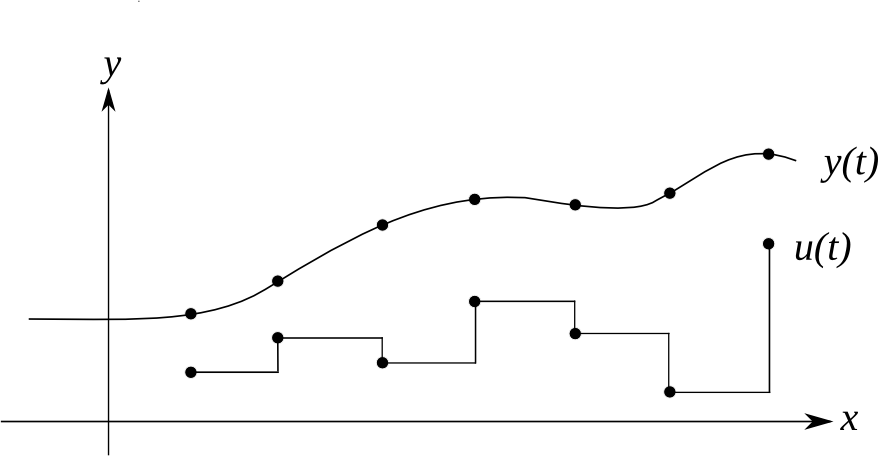
\includegraphics[width=.5\textwidth]{images/03zoh}
	\caption{Input modeled as a zero-order hold (ZOH) signal.}
	\label{fig:03zoh}
\end{figure}

\section{Discrete Time System Representations}
There are four main forms used to represent dyanmic systems:
\begin{itemize}
\item Impulse Response
\item Transfer Function
\item State Space
\item Linear Regression
\end{itemize}

\subsection{Impulse Response Representation}
This system is represented as the total system response to individual impulse functions.
\begin{align*}
y(k\dt) &= G(q)u(k\dt) \\
G(q) &= \sum_{k=0}^\infty g_kq^{-k} \\
q^{-1}u(k) &= u(k-1)
\end{align*}
where $g_k$ is defined as the impulse response or Markov parameters.

\textit{Example:} Let the input be a discrete time pulse function
\begin{align}
\label{eq:03impulse}
u(k) = \begin{cases} 1, & k=0 \\ 0, & k\neq 0 \end{cases}
\end{align}

Then the outputs are
$$y(0)=g_0, ~y(1)=g_1, ~y(2)=g_2, ~\ldots, ~y(n)=g_n$$
This shows that the outputs to impulses are exactly the coefficients used to describe the system.
$\lozenge$

\subsection{BIBO Stability}
BIBO is bounded input bounded output and is achieved when the Markov parameters satisfy the relationship
$$\sum_{k=0}^\infty |g_k| < \infty \Rightarrow \lim_{N\to \infty} g_N \to 0$$
There is a stronger statement for strict BIBO stability that can be made when
$$\sum_{k=0}^\infty k|g_k| < \infty$$
To have strict BIBO stability the individual Markov parameters must have $g_k=k^{-d}$, $d=1$ for the product $k|g_k|\to 0$ or $g_k=\lambda$ where $|\lambda|<1$. The second case is the one encountered most often in this course.

\subsection{Transfer Function Representation}
The dynamics of the system are described by $g_k$ above, but there are an infinite number of those parameters. In this course we will restrict the systems studied to those described by two polynomials.
$$\sum_{k=0}^\infty g_kq^{-k} = q^{-l} \frac{b_0 + b_1q^{-1} + \cdots + b_nq^{-n}}{1+a_1q^{-1} + \cdots + a_nq^{-n}}$$
where $l$ is the amount of delay in the system. Determining those coefficients is done by applying an impulse input to the system and measuring the output. However, it is not clear that $g_k$ can be described by a finite set of coefficients.

The delay is described by $y(k) = G(q)u(k)$ and
$$y(k) + a_1y(k-1)+\cdots + a_ny(k-n) = b_0u(k-l)+b_1u(k-1-l) + \cdots + b_nu(k-n-l)$$
This form is much easier to use for computation of the $a_i$ and $b_i$ coefficients. It is also possible to write the output as
$$y(k) = b_0u(k-1) + b_1u(k-1-l) + \cdots + b_nu(k-n-l) - a_1y(k-1) - \cdots - a_ny(k-n)$$

If $a_i=0$, $i=0,1,2,\ldots,n$ then the sum of Markov parameters is finite, where $g_0=b_0, ~g_1=b_1, ~g_2=b_2, ~\ldots, ~g_n=b_n$. This means that the memory of the system is finite, where the memory of the system is embedded in the $a_i$ coefficients.

\textit{Example:} Let
\begin{align*}
&G(q) = \frac{1}{1+a_1q^{-1}} \\
&y(k) = G(q)u(k) = \frac{1}{1+a_1q^{-1}}u(k) \\
&\Rightarrow (1+a_1q^{-1})y(k) = u(k) \\
&\Rightarrow y(k) = u(k) - a_1y(k-1)
\end{align*}
where the last equation is known as a "difference equation". How do we then re-write this as an infinite sum of Markov parameters? Apply the impulse input from (\ref{eq:03impulse}) to get the parameters as
\begin{align*}
y(0) &= u(0) - a_1y(-1) = 1-1 = 1 \\
y(1) &= u(1) - a_1y(0) = 0 - a_1 \cdot 1 = -a_1 \\
y(2) &= u(2) - a_1y(1) = a_1^2 \\
y(3) &= u(3) - a_1y(2) = -a_1^3 \\
\vdots & \\
g_k &= (-1)^ka_1^k
\end{align*}
and the system is BIBO stable iff $|a_1|<1$, and since there is an exponential it is automatically strictly BIBO stable because the exponential function will "win" over the linear function of $k$.
$\lozenge$
\begin{figure}[ht!]
	\centering
	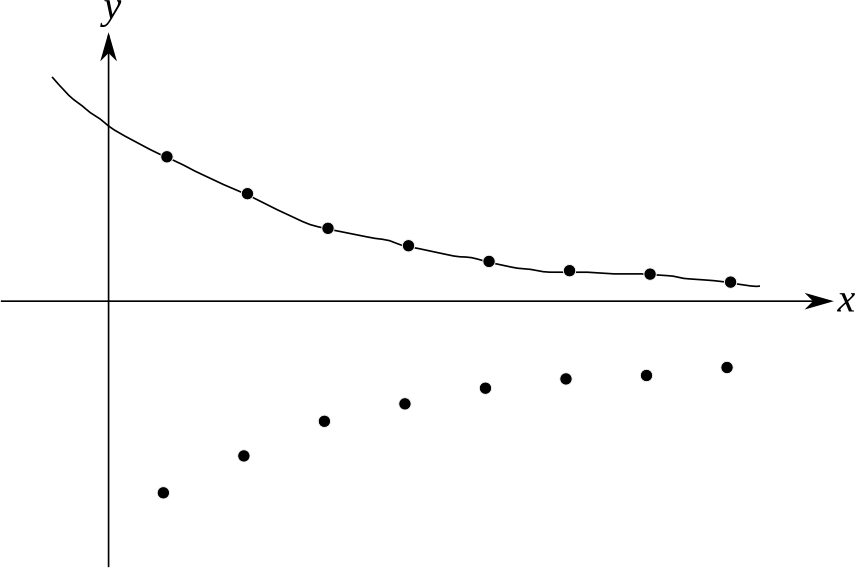
\includegraphics[width=.5\textwidth]{images/03markovParams}
	\caption{Markov parameters. Points are for $0<a_1<1$ and the line is for $|a_1|<1, a_1<0$.}
	\label{fig:03markovParams}
\end{figure}

\subsection{State Space Representation}
Let the system description be
\begin{align*}
x(k+1) &= Ax(k) + Bu(k) \\
y(k) &= Cx(k) + Du(k)
\end{align*}

How do we go from state space to transfer function representation? Use
\begin{align*}
&qx(k) = Ax(k) + Bu(k) \\
&(qI-A)x(k) = Bu(k) \\
&x(k) = (qI-A)^{-1}Bu(k) \\
&y(k) = (C(qI-A)^{-1}B+D)u(k)
\end{align*}
where we let $G(q) = (C(qI-A)^{-1}B+D$.

How do we go from state space to impulse response representation? Recall that the IR is $\sum_{k=0}^\infty g_kq^{-k}$. By applying an impulse response from (\ref{eq:03impulse}) as input to get
\begin{align*}
y(0) &= Cx(0) + Du(0) = D \\
x(1) &= Ax(0) + Bu(0) = B \\
y(1) &= Cx(1) + Du(1) = CB \\
x(2) &= Ax(1) + Bu(1) = AB \\
y(2) &= Cx(2) + Du(2) = CAB \\
x(3) &= Ax(2) + Bu(2) = A^2B \\
y(3) &= Cx(3) + Du(3) = CA^2B \\
&\vdots \\
g_k &= \begin{cases} D, & k=0 \\ CA^{k-1}B, & k\neq 0 \end{cases}
\end{align*}

\subsection{Linear Regression Representation}
Let the system description be
$$y(t)=\phi^T(t)\theta = \theta^T\phi(t)$$
where $\phi(t)$ is the regressor and $\theta$ is the parameter. Typically, $\phi(t)$ contains past inputs and outputs.
\begin{align*}
\begin{split}
\phi(t) = \left[\begin{array}{c}
			u(k) \\
			u(k-1) \\
			\vdots \\
			u(k-n) \\
			-y(k-1) \\
			\vdots \\
			-y(k-n)
		\end{array}\right],
\end{split}
\begin{split}
\theta = \left[\begin{array}{c}
			b_0 \\
			b_1 \\
			\vdots \\
			b_n \\
			a_1 \\
			a_2 \\
			\vdots \\
			a_n
		\end{array}\right]
\end{split}
\end{align*}
Writing out the product gives
$$y(k) = G(q)u(k), ~ G(q) = \frac{b_0+b_1q^{-1}+\cdots+b_nq^{-n}}{1+a_1q^{-1}+\cdots+a_nq^{-n}}$$
Linear regression makes it easy to modify elements of $\phi(t)$ to make the system description non-linear. Possibilities include squaring some of the elements or multiplying two elements to get a new element.

\section{Summary}
\subsection{Impulse Response}
$G(q) = \sum_{k=0}^\infty$, with BIBO stability if $\sum_{k=0}^\infty |g_k| < \infty$ and strict BIBO stability if $\sum_{k=0}^\infty k|g_k| < \infty$.

\subsection{Transfer Function}
$G(q) = \frac{num}{den}$, and assuming no cancellations then the system is strictly BIBO stable if $|\text{roots}\lbrace \text{den}(q)\rbrace|<1$. Figure \ref{fig:03poleMapSZ} shows that the continuous time poles must be $\text{Re}(\cdot) < 0$ and the discrete time poles must be $|(\cdot)| < 1$ for stability.
\begin{figure}[ht!]
	\centering
	\includegraphics[width=.6\textwidth]{images/03poleMapSZ}
	\caption{Mapping of poles from the S-plane to the z-plane.}
	\label{fig:03poleMapSZ}
\end{figure}

\subsection{Laplace Transform}
The Laplace transform allows us to re-write the system as
\begin{align*}
g(s) &= \tint g(t)e^{-st}dt \\
&= \tint g(t)\sum_{k=-\infty}^\infty \delta(t-k\dt)e^{-st}dt \\
&= \sum_{k=-\infty}^\infty g(k\dt)e^{-sk\dt}
\end{align*}
where $z\triangleq e^{s\dt} \Rightarrow g(s) = \sum_{k=-\infty}^\infty g(k\dt)z^{-k}$.

\subsection{z-Transform}
The z-transform can be derived from the $\mathcal{L}$-transform or it can be defined as
$$y(z) = \sum_{k=-\infty}^\infty y(k\dt)z^{-k}, ~z=e^{s\dt}$$
$$z\lbrace qu(k)\rbrace = \sum_{k=-\infty}^\infty u((k+1)\dt)z^{-k} = z\cdot u(z)$$
In this way the time-shift operation becomes multiplication and we also get
$$z\lbrace q^{-1}u(k)\rbrace = z^{-1}\cdot u(z)$$

\subsection{Discrete Time Transfer Function}
$G(q)|_{z=q} = G(z)$

\subsection{z-Transform and System Poles}
$z=e^{s\dt}$ also holds for poles $S$ of a continuous time system converted to discrete time using the ZOH input signal.
$$z_i=e^{S_i\dt}, ~ S_i = a_i+jb_i \Rightarrow z_i = e^{a_i\dt} \cdot e^{jb_i\dt}$$
For stability $|z_i|<1$, $|z_i|=\left| e^{a_i\dt}\right|$. See Figure \ref{fig:03poleMapSZ} for pole ranges. For very small $\dt$ the poles become ill-conditioned as seen in Figure \ref{fig:03poleMapSZsmallT}.
\begin{figure}[ht!]
	\centering
	\includegraphics[width=.6\textwidth]{images/03poleMapSZsmallT}
	\caption{Mapping of poles from the S-plane to the z-plane when $\dt$ is small.}
	\label{fig:03poleMapSZsmallT}
\end{figure}

\subsection{Frequency Response}
In continuous time the system can be modeled as $G(s)|_{s=j\w}\to|G(j\w)|$. And in discrete time the system model $G(z)|_{z=e^{j\w\dt}}$ is periodic with period $\frac{2\pi}{\dt}$. Also, $G(e^{j\w\dt}) = \overline{G(e^{-j\w\dt)}}$ means that we  \textit{still} only need to plot the function over the range $[0, \frac{\pi}{2}]$, where the Nyquist frequency is $\w_N=\frac{\pi}{2}$. When the functions are plotted outside of this range it looks unprofessional.

\subsection{Ljung Notation}
In the textbook by Ljung it always uses $\dt=1$ in discrete time and does so without loss of generality. This means that $u(k\dt) = u(k)$. The book uses $u(t)$ for $u(k)$, where $t=0,1,2,\ldots,n$. Try not to get confused.


\end{document}

%%%%%%%%%%%%%%%%%%%%%%%%%%%%%%%%%%%%%%%%%%%%%%%%%%%%%%%%%%%%%